\documentclass{beamer}
%\usepackage[T1]{fontenc}
\usepackage[utf8]{inputenc}
%\usepackage{lmodern}  % Use the Latin Modern font family

\usepackage{latexsym,amsmath,xcolor,bm, amssymb, color, tikz, graphicx, amsthm, mathtools}
\usepackage{algorithm}
\usepackage{algorithmic}
\usepackage{hyperref}
\usepackage{float}     
\usepackage{CJKutf8}
\usepackage{multicol}
\usepackage{verbatim}

\graphicspath{{../logos/}}

\DeclareMathOperator*{\argmax}{arg\,max}
\DeclareMathOperator*{\argmin}{arg\,min}
\DeclareMathOperator{\sign}{sign}
\DeclareMathOperator{\Tr}{Tr}

\makeatletter
\DeclareRobustCommand\onedot{\futurelet\@let@token\@onedot}
\def\@onedot{\ifx\@let@token.\else.\null\fi\xspace}
\def\eg{\emph{e.g}\onedot} 
\def\Eg{\emph{E.g}\onedot}
\def\ie{\emph{i.e}\onedot} 
\def\Ie{\emph{I.e}\onedot}
\def\cf{\emph{c.f}\onedot} 
\def\Cf{\emph{C.f}\onedot}
\def\etc{\emph{etc}\onedot} 
\def\vs{\emph{vs}\onedot}
\def\wrt{w.r.t\onedot} 
\def\dof{d.o.f\onedot}
\def\etal{\emph{et al}\onedot}
\makeatother


\usetheme{Madrid}
\useinnertheme{circles}


\definecolor{ColorUNLP}{HTML}{8c0011} 
\usecolortheme[named=ColorUNLP]{structure}
%\usecolortheme[named=ColorUNR]{exampleblock}

%\setbeamertemplate{blocks}[rounded][shadow=true]
%\setbeamercolor{block body}{fg=black,bg=white}



%------------------------------------------------------------
%This block of code defines the information to appear in the
%Title page
\title %optional
{Introducción a la Programación Competitiva}

\subtitle{Inicial}

%\subtitle{with applications to persuation and lie production}
% \author % (optional)
% {Author Name}

\author[Matías Ramos]{Matías Ramos}

\institute[]{Universidad Tecnológica Nacional – Facultad Regional Santa Fe}
\date[TC 2026]{Training Camp 2026}
\titlegraphic{
\includegraphics[clip,height=2cm,keepaspectratio]{logoTC.pdf}}

%End of title page configuration block
%------------------------------------------------------------


%------------------------------------------------------------
% \AtBeginSection inserts an automatic Outline slide at the start of
% each \section{}, highlighting the current section. Change the
% \section names below to your real topic names and these slides
% will update automatically.
\AtBeginSection[]
{
  \begin{frame}
    \frametitle{Outline}
    \tableofcontents[currentsection]
  \end{frame}
}
%------------------------------------------------------------


\begin{document}


%The next statement creates the title page.
\frame{\titlepage}


%------------------------------------------------------------
% Frame de Sponsors, me parece mejor ponerlo al principio
% Antes del índice/contenido

% --- Organizadores y Sponsors ---
\begin{frame}{Gracias Sponsors!}
    \begin{columns}[t]
        \column{0.5\textwidth}
        \centering
        Organiza\\
        \vspace{0.5cm}
        
\includegraphics[width=0.6\textwidth,keepaspectratio]{logo_aapc.png}\\
        \vspace{0.3cm}
        
\includegraphics[width=0.8\textwidth,keepaspectratio]{unlp_informatica.png}
        \column{0.5\textwidth}
        \centering
        Diamond Sponsor\\
        \vspace{0.5cm}
        
\includegraphics[width=0.8\textwidth,keepaspectratio]{GTSlogo.jpeg}
    \end{columns}
\end{frame}


%---------------------------------------------------------
%This block of code is for the table of contents after
%the title page
\begin{frame}
\frametitle{Outline}
\tableofcontents
\end{frame}
%---------------------------------------------------------


% ============================================================
% Reemplazar el nombre de la sección con el tema de la clase.
% ============================================================
\section{Presentacion}

\begin{frame}{como competidor}
  \begin{center}
    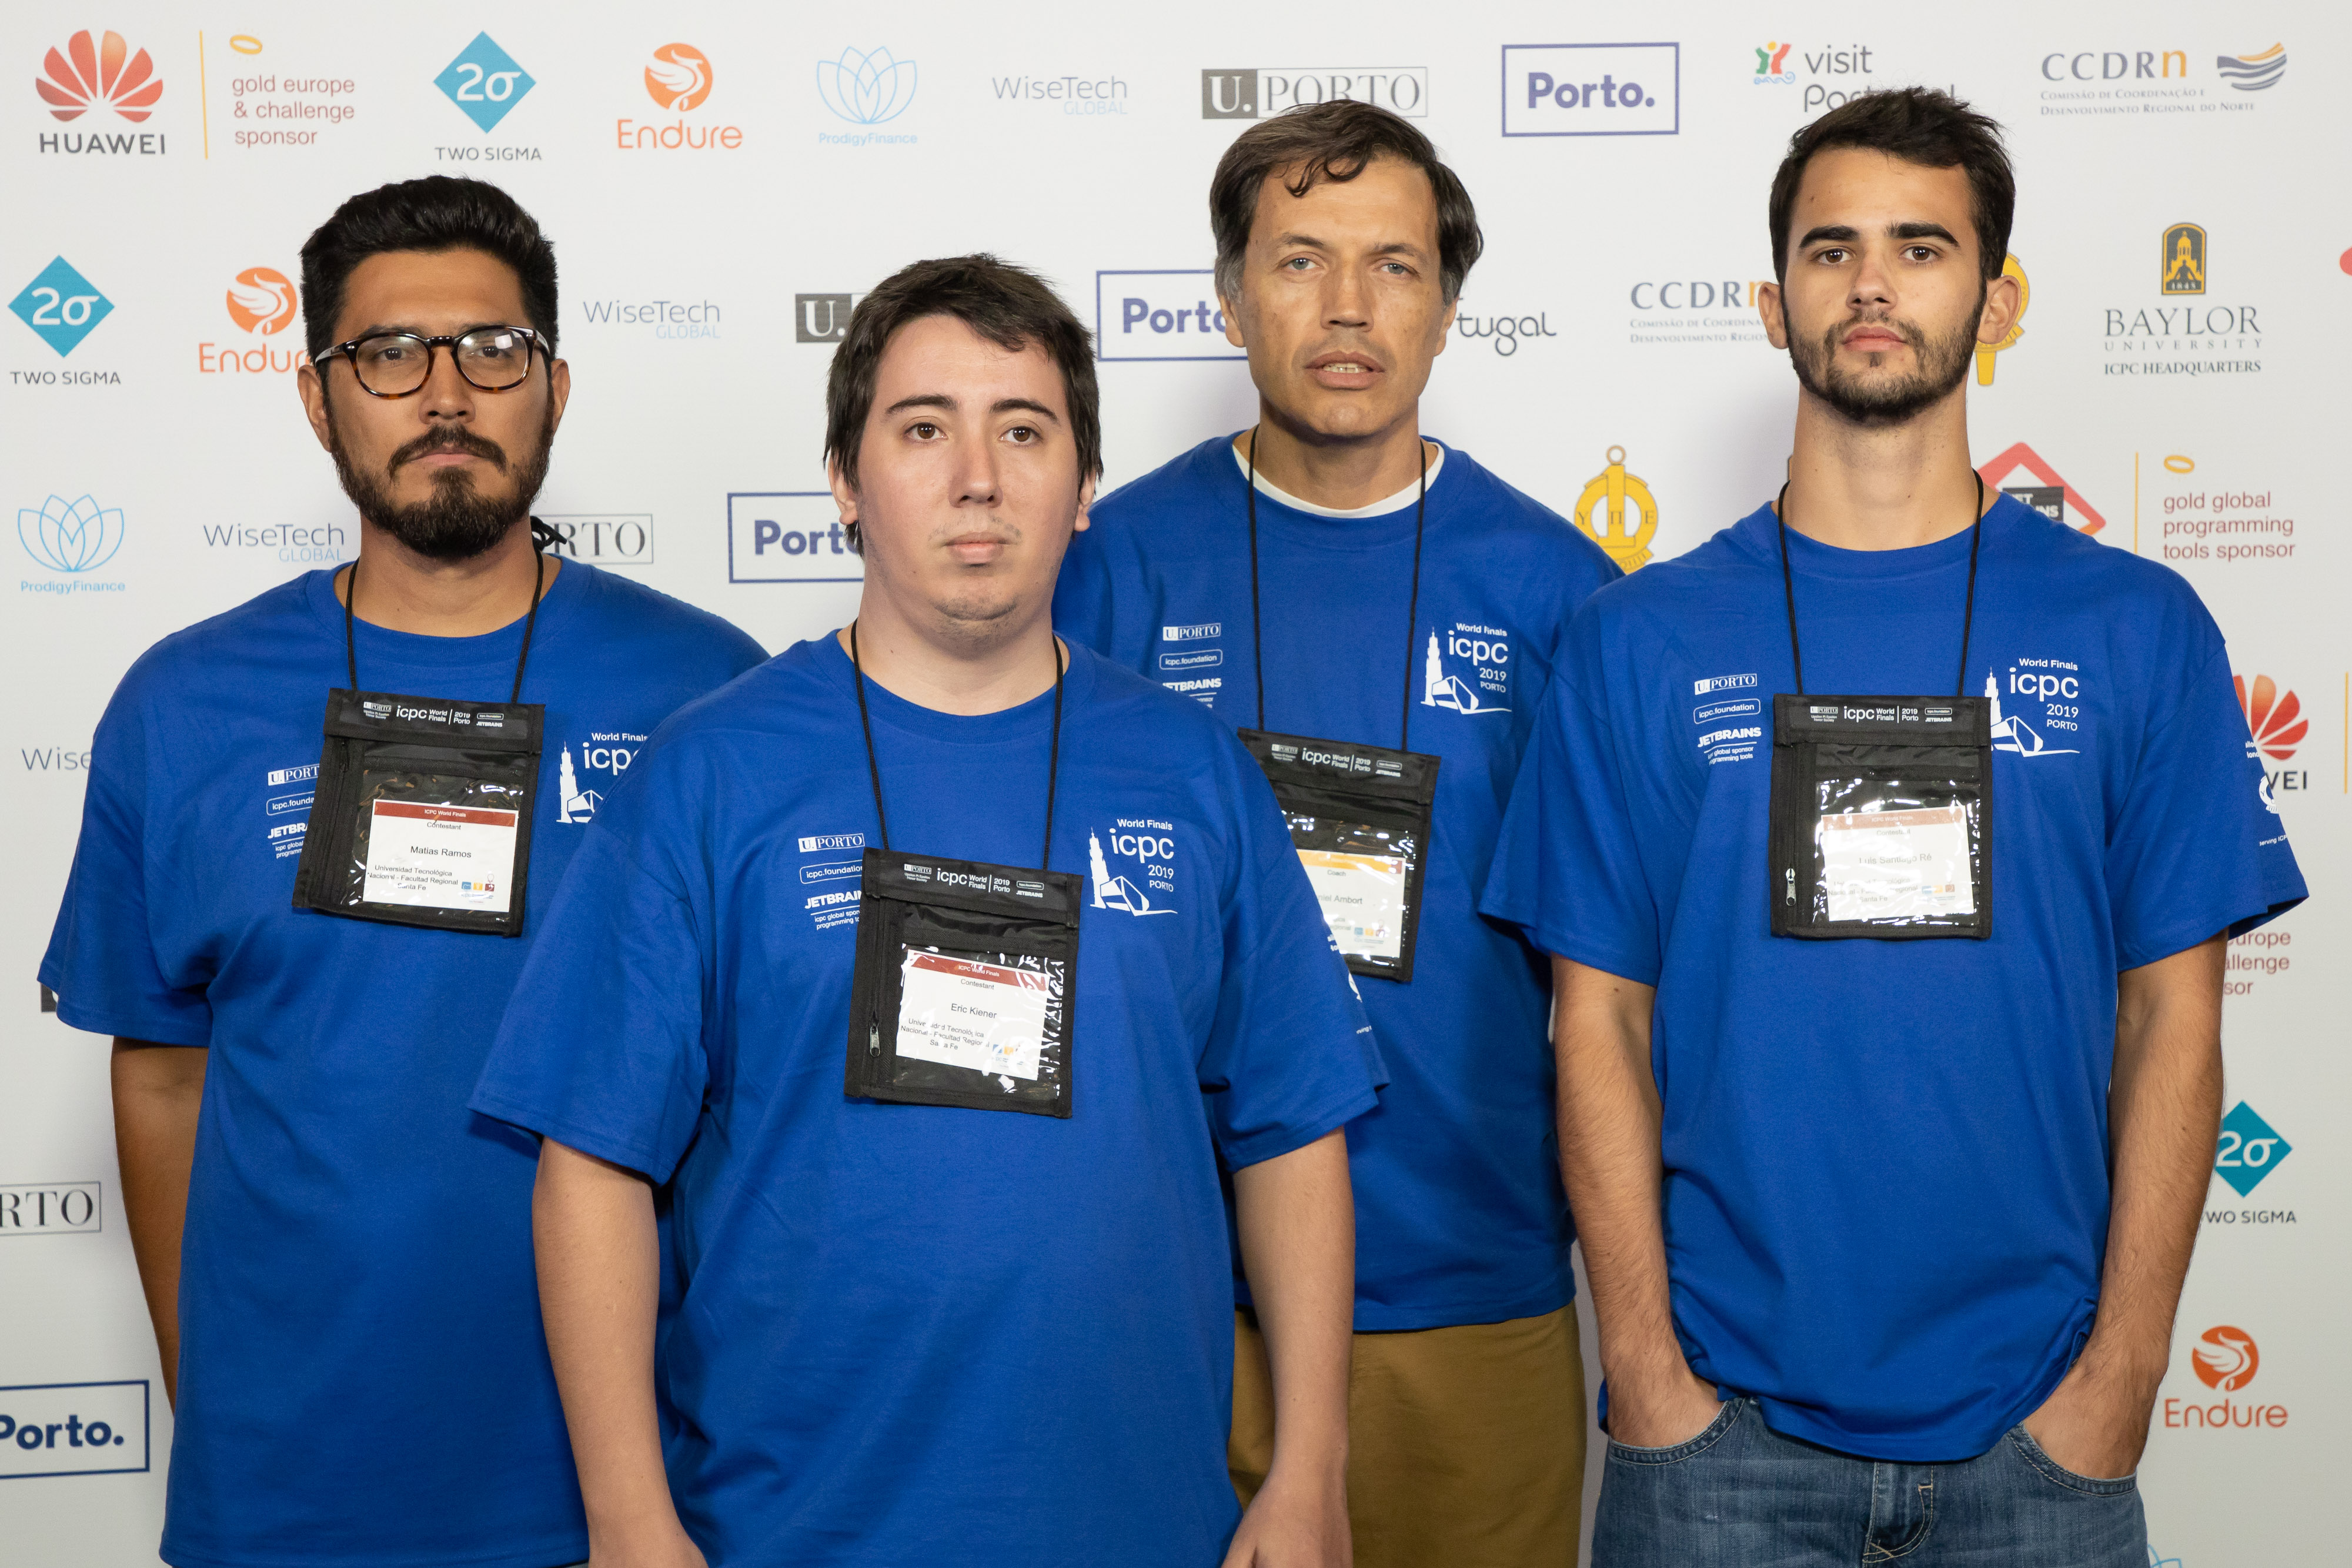
\includegraphics[width=0.75\textwidth,height=0.7\textheight,keepaspectratio]{fotos/competidor.jpg} \\
    \vspace{0.2cm}
    \small Porto 2019
  \end{center}
\end{frame}

\begin{frame}{como coach}
  \begin{center}
    \begin{tabular}{ccc}
      \begin{minipage}{0.25\textwidth}
        
\includegraphics[width=\linewidth]{fotos/anarap.png} \\
        \centering \scriptsize Anarap (Egipto '24)
      \end{minipage}
      &
      \begin{minipage}{0.25\textwidth}
        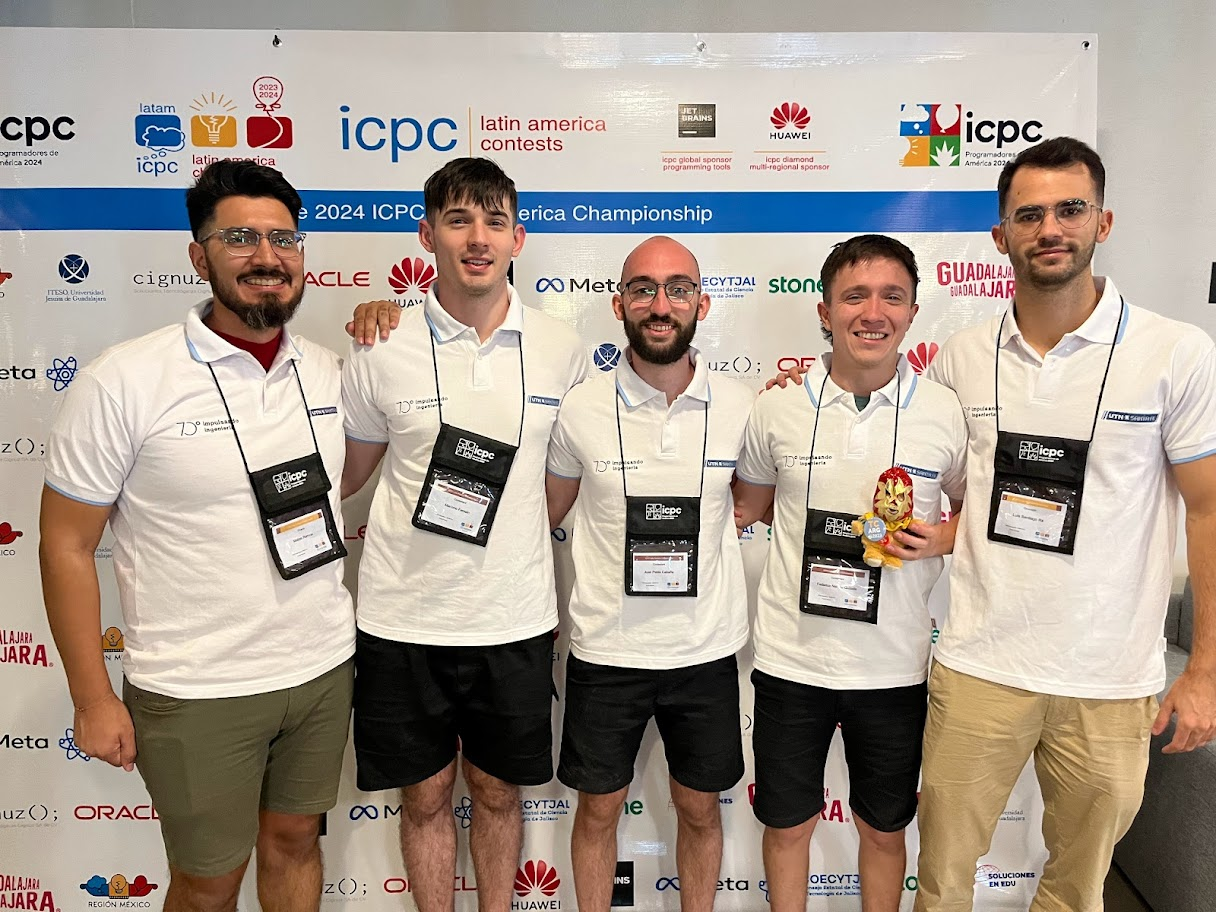
\includegraphics[width=\linewidth]{fotos/mexico.jpg} \\
        \centering \scriptsize Fruta Fresca (México '24)
      \end{minipage}
      &
      \begin{minipage}{0.25\textwidth}
        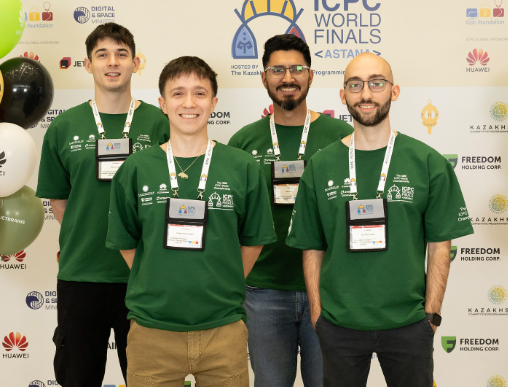
\includegraphics[width=\linewidth]{fotos/kazajistan.png} \\
        \centering \scriptsize \makebox[0.95\linewidth]{Fruta~Fresca~(Kazajistán~'24)}
      \end{minipage}
    \end{tabular}
    
    \vspace{0.3cm}
    
    \begin{tabular}{cc}
      \begin{minipage}{0.25\textwidth}
        
\includegraphics[width=\linewidth]{fotos/champan.png} \\
        \centering \scriptsize \makebox[0.95\linewidth]{Champán~en~Lata~(Brasil~'25)}
      \end{minipage}
      &
      \begin{minipage}{0.25\textwidth}
        \includegraphics[width=\linewidth]{fotos/coach.jpg} \\
        \centering \scriptsize \makebox[0.95\linewidth]{Champán~en~Lata~(Chile~'26)}
      \end{minipage}
    \end{tabular}
  \end{center}
\end{frame}



\section{¿Qué es un problema?}

\begin{frame}
  \frametitle{¿Qué es un problema?}

  \textbf{Problema de ejemplo:}
  
  Juan tiene $0 \leq X \leq 90$ manzanas, y quiere repartirlas entre $0 \leq Y \leq 10$ amigos. \\
  Suponiendo que quiere maximizar la cantidad de manzanas que reparte, y que todos reciban la misma cantidad,\\
  ¿cuántas manzanas recibiría cada uno?

  \textbf{Input:}

  2 \\
  15 2 \\
  17 5 \\

  \textbf{Output:}

  7 \\
  5 \\

\end{frame}


\section{Operaciones}

\begin{frame}
  \frametitle{Operaciones}

  \textbf{¿Cuántas operaciones entran en tiempo?}

  Podemos dividir en tres secciones:
  
  \begin{itemize}
    \item \textcolor{green!60!black}{\textbf{$\leq 10^8$ operaciones}}: Siempre entran en 1 segundo.
    \item \textcolor{orange!90!black}{\textbf{Entre $10^8$ y $10^9$ operaciones}}: Puede funcionar, dependerá principalmente de qué hace cada operación.
    \item \textcolor{red}{\textbf{$> 10^9$ operaciones}}: \textbf{PELIGRO}: casi siempre lleva a \texttt{TIME LIMIT}.
  \end{itemize}

\end{frame}

\begin{frame}
  \frametitle{Notación Big O ($\mathcal{O}$)}
  \textbf{¿Qué es y para qué sirve?}
  \begin{itemize}
    \item Nos permite estimar de manera abstracta el \textbf{tiempo de ejecución} (o memoria) de un algoritmo en el \textbf{peor caso}.
    \item Expresa cómo crece el número de operaciones en función del tamaño de la entrada ($N$).
    \item \textbf{Regla fundamental:} Despreciamos constantes y términos de menor orden. 
    \begin{itemize}
      \item Ejemplo: $3N^2 + 5N + 10 \Rightarrow \mathcal{O}(N^2)$
    \end{itemize}
  \end{itemize}
  
  \vspace{0.2cm}
  \textbf{Ejemplos intuitivos:}
  \begin{itemize}
    \item $\mathcal{O}(1)$: Acceso directo en un vector.
    \item $\mathcal{O}(\log N)$: Búsqueda binaria (dividir el problema a la mitad).
    \item $\mathcal{O}(N)$: Recorrer un arreglo con un solo bucle.
  \end{itemize}
\end{frame}

\begin{frame}{Complejidades Comunes en CP}
  \textbf{¿Qué complejidad usar según los límites del problema?}
  
  Para un límite de tiempo de 1 segundo ($\approx 10^8$ operaciones):
  
  \begin{table}
    \centering
    \small
    \setlength{\tabcolsep}{4pt}
    \begin{tabular}{|l|c|l|}
      \hline
      \textbf{Complejidad} & \textbf{Límite típico de $N$} & \textbf{Algoritmo / Ejemplo} \\
      \hline
      $\mathcal{O}(1)$ & $10^{18}$ & Fórmulas matemáticas, acceso directo \\
      $\mathcal{O}(\log N)$ & $10^{18}$ & Búsqueda binaria \\
      $\mathcal{O}(N)$ & $10^8$ & Bucle simple, Two pointers \\
      $\mathcal{O}(N \log N)$ & $10^6$ & Ordenamiento (std::sort), Segment Tree \\
      $\mathcal{O}(N^2)$ & $5000$ & Bucles anidados, DP simple \\
      $\mathcal{O}(N^3)$ & $500$ & Multiplicación de matrices \\
      $\mathcal{O}(2^N)$ & $20$ & Backtracking, fuerza bruta \\
      $\mathcal{O}(N!)$ & $10$ & Permutaciones de un arreglo \\
      \hline
    \end{tabular}
  \end{table}
\end{frame}

\begin{frame}
  \frametitle{Límites y Overflow}

  \textbf{Los tipos de datos tienen sus límites también:}

  \begin{itemize}
    \item \texttt{int} $\Rightarrow$ desde $-2^{31}$ hasta $2^{31}-1$ ($\approx \pm 2 \cdot 10^{9}$).
    \item \texttt{long long} $\Rightarrow$ desde $-2^{63}$ hasta $2^{63}-1$ ($\approx \pm 9 \cdot 10^{18}$).
  \end{itemize}

  \vspace{0.3cm}
  \textbf{Al superar esos límites, llegamos al famoso \textcolor{red}{\texttt{OVERFLOW}}.}

\end{frame}


\begin{frame}
  \frametitle{¿Cómo evitar el overflow?}

  \textbf{El overflow es un error \textcolor{red}{MUY COMÚN}.}

  \vspace{0.2cm}
  El uso de \textbf{aritmética modular} (A.K.A. operaciones MOD) es fundamental:  

  \begin{itemize}
    \item \texttt{\%} (MOD): devuelve el resto de una división.
    \item \texttt{ADD mod}: $(a + b) \bmod m$
    \item \texttt{SUB mod}: $(((a - b) \bmod m) + m ) \bmod m$
    \item \texttt{MUL mod}: $(a \cdot b) \bmod m$
  \end{itemize}

  \vspace{0.2cm}
  \textbf{Recomendaciones:}
  \begin{itemize}
    \item Usar tipos de 64 bits: \texttt{long long} en C++.
    \item Es mejor usar \texttt{MOD} de más que de menos.
  \end{itemize}

\end{frame}



\section{Estructuras útiles}


\begin{frame}
  \frametitle{Operaciones útiles}

  \textbf{Operaciones comunes:}
  \begin{itemize}
    \item \texttt{sort(v.begin(), v.end(), comparador);}
    \item 
    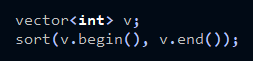
\includegraphics[width=0.4\textwidth]{fotos/sort.png}
    \item \texttt{lower\_bound(v.begin(), v.end(), x);} (requiere orden)
    \item \texttt{set.lower\_bound(x);} (asi se usa en sets)
    \item \texttt{upper\_bound();}
  \end{itemize}
\end{frame}


\begin{frame}
  
  \frametitle{Estructuras importantes}
  Hay algunas estructuras que son \textbf{muy importantes}:
  \begin{itemize}
    \item \texttt{vector}
    \item \texttt{queue}
    \item \texttt{deque}
    \item \texttt{set}
    \item \texttt{map}
  \end{itemize}
\end{frame}



\begin{frame}
  \frametitle{Vector}
  \begin{itemize}
    \item \texttt{vector<T>} en C++, con \texttt{push\_back} y \texttt{pop\_back}
    \item \texttt{ArrayList<T>} en Java, con \texttt{add} y \texttt{remove(list.size()-1)}
    \item \texttt{list} en Python, con \texttt{append} y \texttt{pop}
    \item Acceso con \texttt{v[pos]} o \texttt{v.get(pos)}
    \item Todas estas operaciones son \textbf{O(1)}
  \end{itemize}
\end{frame}

\begin{frame}
  \frametitle{Queue}
  \begin{itemize}
    \item \texttt{queue<T>} en C++, con \texttt{push}, \texttt{front}, \texttt{pop}
    \item \texttt{ArrayDeque<T>} en Java, con \texttt{add}, \texttt{getFirst}, \texttt{remove}
    \item \texttt{collections.deque} en Python, con \texttt{append}, \texttt{deque[0]}, \texttt{popleft}
    \item Se comporta como una cola (FIFO)
    \item Operaciones en \textbf{O(1)}
  \end{itemize}
\end{frame}

\begin{frame}
  \frametitle{Deque}
  \begin{itemize}
    \item \texttt{deque<T>} en C++, con \texttt{push\_front}, \texttt{push\_back}, \texttt{pop\_front}, \texttt{pop\_back}
    \item \texttt{ArrayDeque<T>} en Java, con \texttt{addFirst}, \texttt{addLast}, \texttt{removeFirst}, \texttt{removeLast}
    \item \texttt{collections.deque} en Python, con \texttt{appendleft}, \texttt{append}, \texttt{popleft}, \texttt{pop}
    \item Acceso en \textbf{O(1)}
    \item Todas las operaciones anteriores son también \textbf{O(1)}
  \end{itemize}
\end{frame}

\begin{frame}
  \frametitle{Set}
  \begin{itemize}
    \item \texttt{set<T>} en C++
    \item \texttt{TreeSet<T>} en Java
    \item En Python no hay un equivalente ordenado nativo
    \item Mantiene elementos \textbf{únicos y ordenados}
    \item Permite insertar, borrar, consultar existencia, \texttt{lower\_bound}, \texttt{upper\_bound}
    \item Todas en \textbf{O(log N)}
    \item Variantes:
    \begin{itemize}
      \item \texttt{unordered\_set} (C++) / \texttt{HashSet} (Java): O(1) amortizado
      \item \texttt{multiset}: permite elementos repetidos
    \end{itemize}
  \end{itemize}
\end{frame}

\begin{frame}
  \frametitle{Map}
  \begin{itemize}
    \item \texttt{map<K, V>} en C++
    \item \texttt{TreeMap<K, V>} en Java
    \item En Python: \texttt{collections.OrderedDict} (aproximado)
    \item Mantiene pares \textbf{clave → valor}
    \item Acceder, insertar, borrar en \textbf{O(log N)}
    \item Variante: \texttt{unordered\_map} (hash, O(1) amortizado)
  \end{itemize}
\end{frame}


\section{Prefix Sum}
\begin{frame}
  \frametitle{Prefix Sum}

  Dado un vector $V$, queremos poder calcular rápidamente la suma de los primeros $X$ elementos, o de cualquier subarreglo.

  \vspace{0.3cm}
  Para eso construimos un \textbf{vector auxiliar} $P$ de tamaño $n+1$, donde:
  \[
    P[i] = V[0] + V[1] + \dots + V[i-1]
  \]

  \vspace{0.3cm}
  \textbf{Ejemplo:}  

  $V = [2,\ 6,\ 2,\ 5,\ 10]$  

  $P = [0,\ 2,\ 8,\ 10,\ 15,\ 25]$

  \vspace{0.3cm}
  Entonces, la suma del subarreglo $V[l\,..\,r]$ se puede calcular en $\mathcal{O}(1)$ como:
  \[
    P[r+1] - P[l]
  \]
\end{frame}

\section{Entrada y salida}

\begin{frame}{Entrada y salida en C++}
  \textbf{Forma elegante de entrada/salida:}
  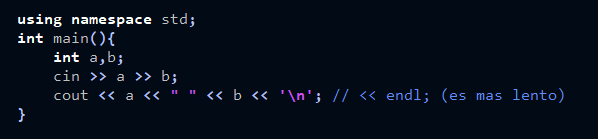
\includegraphics[width=0.8\textwidth,keepaspectratio]{fotos/cin.png}

  \vspace{0.2cm}
  Leer y escribir consume tiempo, por lo tanto hay que tener cuidado.
\end{frame}

\begin{frame}[fragile]{Acelerando entrada/salida}

  \textbf{Recomendaciones en C++:}
  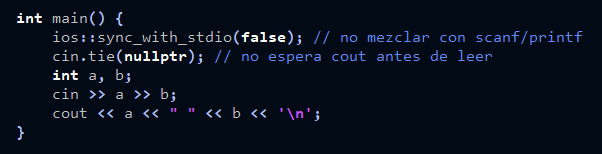
\includegraphics[width=0.8\textwidth,keepaspectratio]{fotos/fastcin.png}
\end{frame}

\section{Uso de Inteligencia Artificial}

\begin{frame}{El Rol Permitido: La IA como Tutor}
  Fuera de las competencias oficiales, usá la IA como un \textbf{"socio de depuración"} y no como un generador de soluciones.
  
  \vspace{0.3cm}
  \textbf{A. Para comprender el problema (sin "spoilers"):}
  \begin{itemize}
    \item \textbf{Traducción y aclaración:} Excelente para interpretar enunciados complejos en inglés técnico o reformular enunciados ambiguos.
    \item \textbf{Modo Socrático:} Pedí pistas, no la solución directa.
    \item \textbf{Prompt recomendado:} 
      \begin{alertblock}{Prompt Clave}
        \scriptsize
        "Explícame este problema de programación competitiva con otras palabras y dame una pista (hint) matemática o algorítmica, pero no me digas el algoritmo final ni me des código."
      \end{alertblock}
  \end{itemize}
\end{frame}

\begin{frame}{Identificar Errores y Stress Testing}
  \textbf{B. Para identificar errores (Debugging efectivo):}
  \begin{itemize}
    \item \textbf{Buscar el contraejemplo:} Si tenés Wrong Answer (WA) en un testcase oculto, en vez de pedir "corregí mi código", pasale el enunciado y tu código e indicá:
      \begin{itemize}
        \item \textit{"¿Qué caso borde (edge case) o desbordamiento de enteros (integer overflow) se me está escapando en este enfoque?"}
      \end{itemize}
    \item \textbf{Generación de Casos de Prueba (Stress Testing):}
      \begin{itemize}
        \item Pedile un script para generar casos de prueba aleatorios o extremos (valores máximos, mínimos, arreglos vacíos).
        \item Compará tu solución rápida que falla contra una lenta pero segura (fuerza bruta).
      \end{itemize}
  \end{itemize}
\end{frame}

\begin{frame}{La Línea Roja: Lo que Prohíben las Plataformas}
  Es vital conocer las reglas actuales para evitar baneos innecesarios (ej. en Codeforces):
  
  \vspace{0.2cm}
  \begin{itemize}
    \item \textbf{Prohibición de Lógica:} No se permite introducir el enunciado para que la IA devuelva el algoritmo exacto o el código a usar.
    \item \textbf{Prohibición de Refactorizar en Competencia:} No se puede copiar el código que falló en un testcase del sistema durante el contest y pedirle a la IA que lo arregle.
    \item \textbf{Uso Limitado de Copilot/Cursor:} Permitido en práctica únicamente para sintaxis repetitiva o boilerplate. Nunca para delegar la lógica central del problema.
  \end{itemize}
\end{frame}

\begin{frame}{Razonamiento Pedagógico: Tu Entrenador Personal}
  \begin{block}{La Analogía del Entrenador}
    Un buen entrenador te enseña a levantar la barra y te corrige la postura (pistas, explicaciones), pero \textbf{si levanta la barra por ti (te da el código funcional), tus músculos no crecen}.
  \end{block}
  
  \vspace{0.2cm}
  \textbf{Regla de Oro:}
  \begin{itemize}
    \item Usá la IA para entender por qué falla un enfoque o desmenuzar enunciados en la fase de práctica.
    \item Nunca la uses para saltarte la frustración del diseño lógico: \textbf{la frustración es el proceso de aprendizaje}.
    \item En la compe presencial (como ICPC) no hay internet ni IA; necesitás desarrollar tu propia intuición algorítmica.
  \end{itemize}
\end{frame}

\section{Consejos personales}

\begin{frame}[fragile]{Consejos personales}
  \begin{itemize}
  \item  Usar una tablita para anotar ideas por problema
  \end{itemize}

  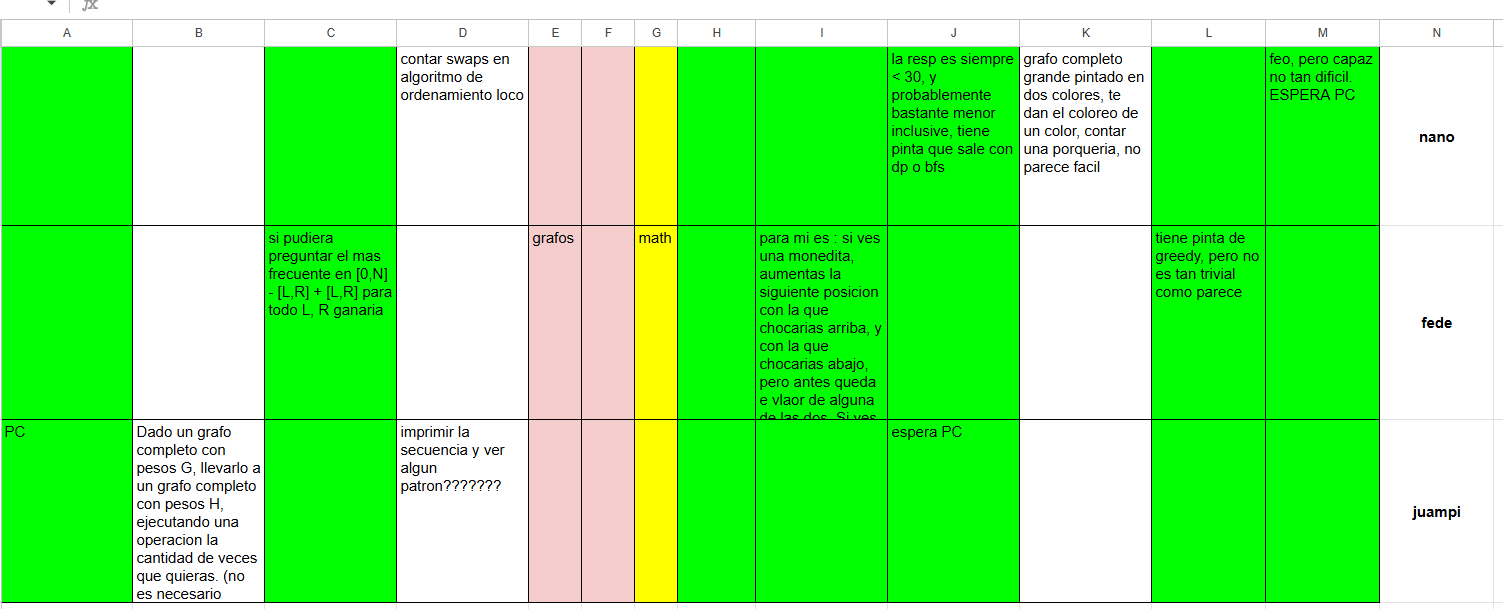
\includegraphics[width=1\textwidth,keepaspectratio]{fotos/tablita.png}

  \begin{itemize}
  \item Aprovechar simulaciones para mejorar la dinámica
  \item Mantener una buena comunicación con el equipo
  \end{itemize}

\end{frame}


\begin{frame}[fragile]{Consejos personales}
  \begin{itemize}
  \item Tener un template útil y propio
  \end{itemize}
  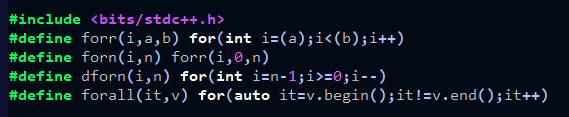
\includegraphics[width=0.8\textwidth,keepaspectratio]{fotos/template.png}

  \begin{itemize}
  \item Acostumbrarse a usar un notebook
  
  \item Aprender a estimar tiempos, antes de resolver
  \end{itemize}
\end{frame}

\begin{frame}[fragile]{Consejos personales}
  \begin{itemize}
  
  \item Asegurarse de entender bien el enunciado, comprobar viendo los ejemplos
  \item Intentar hacer al menos una demo minima de la solucion
  \item Leer editoriales → entender el \textbf{cómo}, no solo el código
  \item Usar IA como herramienta, no como solución (ver sección anterior para más detalle)

  \end{itemize}
\end{frame}



\begin{frame}[fragile]{Consejos personales}
  \begin{itemize}
  \item \textbf{UPSOLVEAR}, esa es la clave
  \end{itemize}
  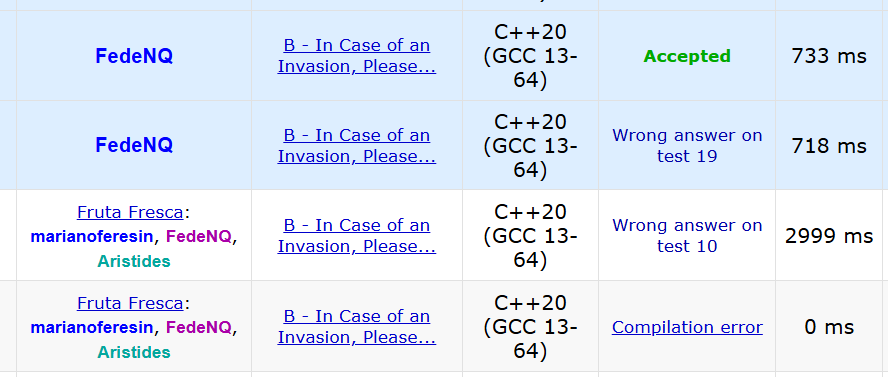
\includegraphics[width=1\textwidth,keepaspectratio]{fotos/uplsoving.png}
  
\end{frame}


\begin{frame}[fragile]{Consejos personales}
  \begin{itemize}
  \item No quedarse con un solo problema, leer otros.
  \item Intentar resolver casos mas simples, ver como mejorar la solucion.
  \item Si los problemas no salen, aprovechen a tomar algunos de los problemas propuestos en las clases.
  \item No tengan miedo de preguntar a los profes/organizadores, les podemos dar una ayudita.
  \item Disfrutar, tanto las competencias como los entrenamientos
  \end{itemize}
  
\end{frame}

\begin{frame}{Problemas Propuestos}
  \textbf{Para practicar los temas de hoy (hacer clic en el título para abrir, seleccionar el texto para ver la pista):}
  
  \begin{itemize}
    \item \href{https://cses.fi/problemset/task/1068}{\underline{\textcolor{blue}{Weird Algorithm}}}: \textcolor{white}{Simulación básica y desbordamiento de enteros (¡ojo con usar \texttt{long long}!).}
    \item \href{https://cses.fi/problemset/task/1083}{\underline{\textcolor{blue}{Missing Number}}}: \textcolor{white}{Sumatoria y lógica básica para encontrar el número faltante.}
    \item \href{https://cses.fi/problemset/task/1094}{\underline{\textcolor{blue}{Increasing Array}}}: \textcolor{white}{Simulación lineal sencilla (requiere acumular la respuesta en \texttt{long long}).}
    \item \href{https://cses.fi/problemset/task/1621}{\underline{\textcolor{blue}{Distinct Numbers}}}: \textcolor{white}{Ordenamiento o uso de \texttt{std::set}.}
    \item \href{https://cses.fi/problemset/task/1646}{\underline{\textcolor{blue}{Static Range Sum Queries}}}: \textcolor{white}{El clásico problema para aplicar \textbf{Prefix Sums}.}
    \item \href{https://cses.fi/problemset/task/1090}{\underline{\textcolor{blue}{Ferris Wheel}}}: \textcolor{white}{Ordenamiento y técnica de dos punteros (o codicia).}
    \item \href{https://cses.fi/problemset/task/1091}{\underline{\textcolor{blue}{Concert Tickets}}}: \textcolor{white}{Búsquedas eficientes con \texttt{lower\_bound} sobre estructuras dinámicas ordenadas.}
  \end{itemize}
  
  \vspace{0.2cm}
  Pueden crearse una cuenta en \href{https://cses.fi/}{cses.fi} para mandar sus soluciones.
\end{frame}

\begin{frame}{Consejos personales}

  \centering
  \large
  Gracias por la atención. \\
  \vspace{0.4cm}
  Suerte en la compe de hoy y en los próximos días. \\
  \vspace{0.4cm}
  Cualquier duda o consulta, tienen mi mail o me buscan por telegram @somartam
  
\end{frame}

\end{document}
